\documentclass [11pt,twoside]{article}
\usepackage[utf8]{inputenc}
\usepackage[T1]{fontenc}

%Page margins, header and footer positions
\usepackage{geometry}
 \geometry{
 a4paper,
 total={210mm,297mm},
 left=25mm,
 right=25mm,
 top=30mm,
 bottom=25mm,
 headsep=7mm}

\interfootnotelinepenalty=10000

%To display filling dots in the TOC for all entries
\usepackage[titles]{tocloft}
\renewcommand{\cftsecleader}{\cftdotfill{\cftdotsep}}

%Define new header and footer style
\usepackage{fancyhdr}

\pagestyle{fancy}
\fancyhf{}
\lhead{\color{Gray}{\small{Travlendar+ project by YOUR NAMES}}}
\lfoot{\textcolor{Gray}{\small{Copyright © 2017, YOUR NAMES – All rights reserved}}}
\rfoot{\textcolor{Gray}{\thepage}}
\renewcommand{\headrulewidth}{0pt}

%PACKAGES
\usepackage{wasysym}
\usepackage{pifont}

\newcommand{\supported}{\ding{52}\xspace}
\newcommand{\unsupported}{\ding{55}\xspace}
\newcommand{\partsupported}{\textcolor{black!40}{\ding{52}}\xspace}
\newcommand{\lowsupported}{\textcolor{black!20}{\ding{52}}\xspace}
\newcommand{\unknowsupported}{\textbf{?}\xspace}

%Font: Times
\usepackage{times}
%Change monospaced font
\renewcommand{\ttdefault}{lmtt}

%tables
\usepackage{tabu}
\usepackage{tabularx}
\usepackage{ltablex}
\usepackage{longtable}
\usepackage{float} % To allow the use of H modifier in long tables

%landscape mode
\usepackage{pdflscape}
\usepackage{rotating}
\usepackage{caption}

%make landscape mode be sensitive to even and odd pages
%start
\def\myrotate{\ifodd\c@page\else-\fi 90}
\makeatletter
\global\let\orig@begin@landscape=\landscape%
\global\let\orig@end@landscape=\endlandscape%
\gdef\@true{1}
\gdef\@false{0}
\gdef\landscape{%
    \global\let\within@landscape=\@true%
    \orig@begin@landscape%
}%
\gdef\endlandscape{%
    \orig@end@landscape%
    \global\let\within@landscape=\@false%
}%
\@ifpackageloaded{pdflscape}{%
    \gdef\pdf@landscape@rotate{\PLS@Rotate}%
}{
    \gdef\pdf@landscape@rotate#1{}%
}
\let\latex@outputpage\@outputpage
\def\@outputpage{
    \ifx\within@landscape\@true%
        \if@twoside%
            \ifodd\c@page%
                \gdef\LS@rot{\setbox\@outputbox\vbox{%
                    \pdf@landscape@rotate{-90}%
                    \hbox{\rotatebox{90}{\hbox{\rotatebox{180}{\box\@outputbox}}}}}%
                }%
            \else%
                \gdef\LS@rot{\setbox\@outputbox\vbox{%
                    \pdf@landscape@rotate{+90}%
                    \hbox{\rotatebox{90}{\hbox{\rotatebox{0}{\box\@outputbox}}}}}%
                }%
            \fi%
        \else%
            \gdef\LS@rot{\setbox\@outputbox\vbox{%
                \pdf@landscape@rotate{+90}%
                \hbox{\rotatebox{90}{\hbox{\rotatebox{0}{\box\@outputbox}}}}}%
            }%
        \fi%
    \fi%
    \latex@outputpage%
}
\makeatother
%end

%graphics
\usepackage{graphicx}
\usepackage[dvipsnames, table]{xcolor}
%If you upload images from PC, you need to insert code for the path here (different for Windows and Unix OS)

%References
%\usepackage{xpatch}
%\usepackage[backend=biber, style=numeric, citestyle=numeric, sorting=none]{biblatex}
%\addbibresource{main.bib}

%Other
\usepackage{ifthen}
\usepackage{xspace}
\usepackage{enumitem}
\usepackage{amssymb}
\usepackage[pdftex, colorlinks]{hyperref}
\newcommand{\comment}[1]{{\color{Red}$\blacktriangleright$ Comment: #1 $\blacktriangleleft$}}


% Some utilities\ldots
\usepackage{soul}
\usepackage{tikz}

\usetikzlibrary{calc}
\usetikzlibrary{decorations.pathmorphing}


\makeatletter

\newcommand{\defhighlighter}[3][]{%
  \tikzset{every highlighter/.style={color=#2, fill opacity=#3, #1}}%
}

\defhighlighter{yellow}{.5}

\newcommand{\highlight@DoHighlight}{
  \fill [ decoration = {random steps, amplitude=1pt, segment length=15pt}
        , outer sep = -15pt, inner sep = 0pt, decorate
       , every highlighter, this highlighter ]
        ($(begin highlight)+(0,8pt)$) rectangle ($(end highlight)+(0,-3pt)$) ;
}

\newcommand{\highlight@BeginHighlight}{
  \coordinate (begin highlight) at (0,0) ;
}

\newcommand{\highlight@EndHighlight}{
  \coordinate (end highlight) at (0,0) ;
}

\newdimen\highlight@previous
\newdimen\highlight@current

\DeclareRobustCommand*\highlight[1][]{%
  \tikzset{this highlighter/.style={#1}}%
  \SOUL@setup
  %
  \def\SOUL@preamble{%
    \begin{tikzpicture}[overlay, remember picture]
      \highlight@BeginHighlight
      \highlight@EndHighlight
    \end{tikzpicture}%
  }%
  %
  \def\SOUL@postamble{%
    \begin{tikzpicture}[overlay, remember picture]
      \highlight@EndHighlight
      \highlight@DoHighlight
    \end{tikzpicture}%
  }%
  %
  \def\SOUL@everyhyphen{%
    \discretionary{%
      \SOUL@setkern\SOUL@hyphkern
      \SOUL@sethyphenchar
      \tikz[overlay, remember picture] \highlight@EndHighlight ;%
    }{%
    }{%
      \SOUL@setkern\SOUL@charkern
    }%
  }%
  %
  \def\SOUL@everyexhyphen##1{%
    \SOUL@setkern\SOUL@hyphkern
    \hbox{##1}%
    \discretionary{%
      \tikz[overlay, remember picture] \highlight@EndHighlight ;%
    }{%
    }{%
      \SOUL@setkern\SOUL@charkern
    }%
  }%
  %
  \def\SOUL@everysyllable{%
    \begin{tikzpicture}[overlay, remember picture]
      \path let \p0 = (begin highlight), \p1 = (0,0) in \pgfextra
        \global\highlight@previous=\y0
        \global\highlight@current =\y1
      \endpgfextra (0,0) ;
      \ifdim\highlight@current < \highlight@previous
        \highlight@DoHighlight
        \highlight@BeginHighlight
      \fi
    \end{tikzpicture}%
    \the\SOUL@syllable
    \tikz[overlay, remember picture] \highlight@EndHighlight ;%
  }%
  \SOUL@
}

\makeatother

% Common abbrev. are set as commands to ensure proper spacing after the dot
\RequirePackage{xspace}
\newcommand{\ie}{i.e.\@\xspace}
\newcommand{\aka}{a.k.a.\@\xspace}
\newcommand{\Ie}{I.e.\@\xspace}
\newcommand{\cf}{cf.\@\xspace}
\newcommand{\Cf}{Cf.\@\xspace}
\newcommand{\eg}{e.g.\@\xspace}
\newcommand{\Eg}{E.g.\@\xspace}
\newcommand{\etal}{et al.\@\xspace}
\newcommand{\etc}{etc.\@\xspace}
\newcommand{\wrt}{w.r.t.\@\xspace}
\newcommand{\Wrt}{W.r.t.\@\xspace}



\date{}


\begin{document}

%TITLE PAGE

%LOGO

{\begin{titlepage}
    \begin{center}
		
\includegraphics[width=0.4\textwidth]{Images/PolimiLogo.png}
		
		\vspace{0.2cm}
		
		\Large Computer Science and Engineering
		
		\vspace{0.8cm}
	
		\Huge \textbf{DD: Design Document}

		
		\vspace{1.5cm}
		\LARGE Software Engineering 2 Project\\
		\Large Academic year 2021 - 2022\\
		\vspace{1cm}
		22 December 2021\\Version 1.0
		\vspace{3cm}
		
		\large
		\begin{minipage}{.1\textwidth}
			\null
		\end{minipage}%
		\begin{minipage}{.4\textwidth}
			\textit{Authors}:\\
			Lorenzo IOVINE\\
			Nicola LANDINI\\
            Francesco LEONE
		\end{minipage}%
		\begin{minipage}{.4\textwidth}
			\raggedleft	
			\textit{Professor}:\\
			Matteo Giovanni ROSSI\\
			\phantom{placeholder}
		\end{minipage}%
		\begin{minipage}{.1\textwidth}
			\null
		\end{minipage}
	
			
		\end{center}
\end{titlepage}}~\\ 

%TITLE 

%Define deliverable specific info
%Replace cell contents where needed
\begin{table}[h!]
\begin{tabu} to \textwidth { X[0.3,r,p] X[0.7,l,p] }
\hline

\textbf{Deliverable:} & DD\\
\textbf{Title:} & Design Document \\
\textbf{Authors:} & Lorenzo Iovine, Nicola Landini, Francesco Leone\\
\textbf{Version:} & 1.0 \\ 
\textbf{Date:} & 09-January-2022 \\
\textbf{Download page:} & https://github.com/fraleone99/IovineLandiniLeone \\
\textbf{Copyright:} & Copyright © 2021, Lorenzo Iovine, Nicola Landini, Francesco Leone – All rights reserved \\
\hline
\end{tabu}
\end{table}




\setcounter{page}{2}


%------------------------------------------------------------------------------------------------------------------------------------------------
\newpage
\addcontentsline{toc}{section}{Table of Contents}
\tableofcontents
\newpage
\addcontentsline{toc}{section}{List of Figures}
\listoffigures
\addcontentsline{toc}{section}{List of Tables}
\listoftables

%------------------------------------------------------------------------------------------------------------------------------------------------
\clearpage
{\color{Blue}{\section{Introduction}}}
\label{sect:introduction}
\subsection{Purpose}
The covid-19 pandemic has greatly highlighted the need of building a resilient food system in India, 
where agriculture plays a pivotal role. 
This need is increased by the problems due to climate change that will impact everything from productivity to 
livelihoods across food and farm systems and is predicted to result in a 4\%-26\% loss in net farm income towards the end of the century.
In addition, according to Harvard Business Review, food demand is expected to increase between 59\% to 98\% by 2050.\\
For this reason policy makers, citizens, agronomists, and farmers should share data and information to achieve better results 
\\\\
Telangana region is an extended and populous state of India, whose economy is mainly driven by agriculture. 
To address the described above problem, Telangana's government want to design, 
develop and demonstrate anticipatory governance models for food system using digital 
public goods and community-centric approaches to strengthen data-driven policy-making in the state.
\\\\
The application aims to enable the acquisition, communication and combination of data provided by Telangana policymakers, 
farmers and agronomists as:
\begin{itemize}
    \item meteorological forecasts
    \item farmers' production
    \item amount of used water
    \item soil humidity
    \item agronomists' report
\end{itemize}
\bigskip
The product will allow policymakers to identify farmers who are performing well and those who are performing badly. 
As the first ones will receive special incentives and will be asked to provide useful best practices to others. 
Furthermore, the application will provide information regarding the results of the farmers who received help.
\\\\
The product needs to provide farmers the ability to visualize data relevant to them based on their location and type of production. 
Farmers should be also able to insert in the system data about production and any problem they face. 
They should be allowed to request help suggestions by agronomists or other farmers and create forums to discuss with their peers.
\\\\
The application will allow agronomists to insert the area they are responsible for, receive information about requests for help, 
and answer them. Agronomists need to know data about weather forecasts and the best performing farmers in the area; 
they also need to visualize and update daily plan visits of farms.

\subsection{Scope}
To represent the scope of the project we use the "The World and The Machine" model by M. Jackson. 
It contains the events which cannot be observed by the system ("The World"), 
those strictly related to the system ("The Machine"), and those in common between them. 

\newpage
\begin{figure}[H]
    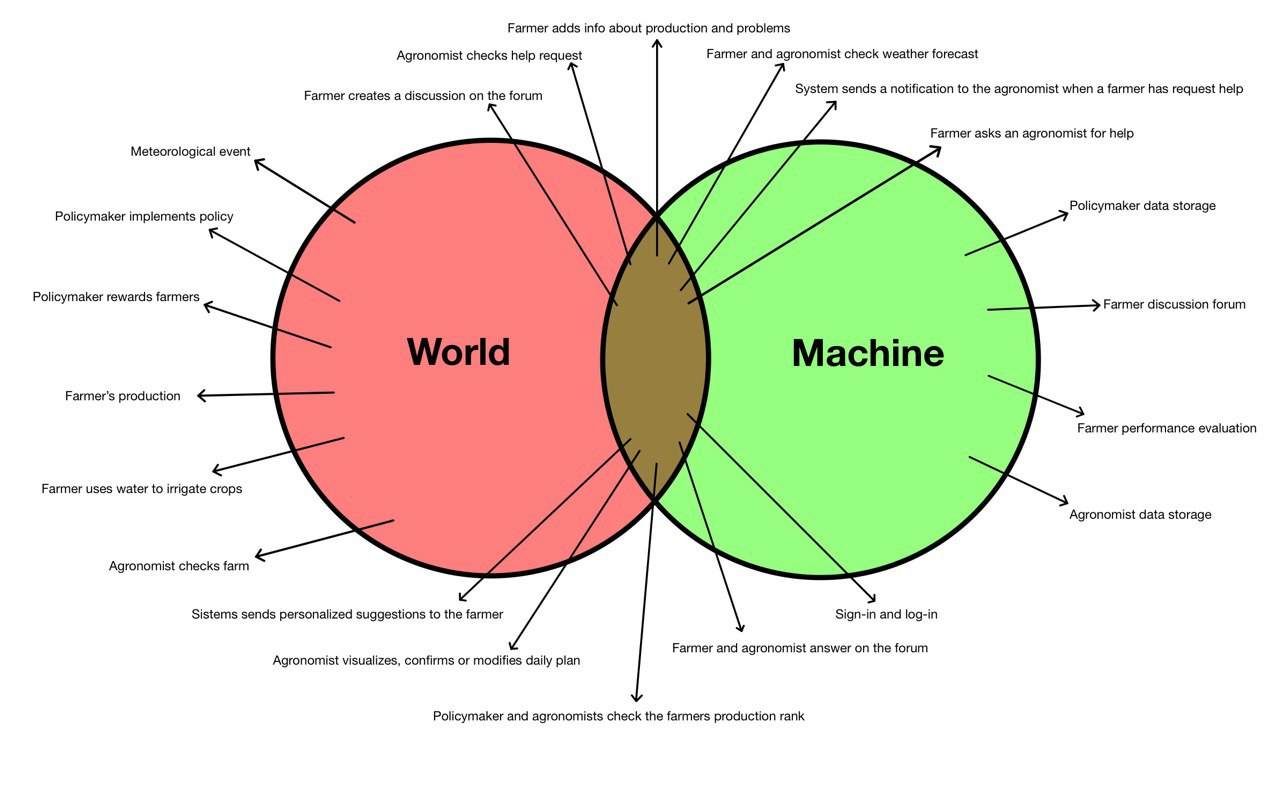
\includegraphics[width=\textwidth,height=\textheight,keepaspectratio]{Images/WorldAndMachine.jpg}
    \caption{The World and the Machine diagram}
    \label{fig:WorldAndMachine}
\end{figure}

\subsubsection{World phenomena}
\begin{itemize}
    \item Meteorological event
    \item Policymaker implements policy
    \item Policymaker rewards farmers
    \item Farmer's production
    \item Farmer uses water to irrigate crops
    \item Agronomist checks farm
\end{itemize}

\subsubsection{Machine phenomena}
\begin{itemize}
    \item Policymaker data storage
    \item Farmer discussion forum
    \item Farmer performance evaluation
    \item Agronomist data storage
\end{itemize}

\subsubsection{Shared phenomena}
\paragraph{Controlled by the World}
\begin{itemize}
    \item Policymaker and agronomist check the farmers production leaderboard
    \item Policymaker sign-in and log-in
    \item Farmer answers help request on the forum
    \item Farmer sign-in and log-in 
    \item Farmer add information about his production
    \item Farmer add information about a problem he faces
    \item Farmer create a discussion on the forum about a problem
    \item Farmer checks weather forecasts
    \item Farmer asks an agronomist for help
    \item Agronomist sign-in and log-in
    \item Agronomist checks help requests
    \item Agronomist answers help request on the forum
    \item Agronomist answers privately help request
    \item Agronomist checks weather forecasts
    \item Agronomist visualizes daily plan
    \item Agronomist confirms or modifies daily plan
\end{itemize}

\paragraph{Controlled by the Machine}
\begin{itemize}
    \item System sends personalized suggestions to the farmer
\end{itemize}

\subsubsection{Goals}

\begin{description}
    \item [G1] Policymakers shall be able to know if steering initiative produced significant results
    \item [G2] Policymakers shall be able to know the best and the worst farmer
    \item [G3] Farmers shall be able to communicate with peers
    \item [G4] Farmers shall be able to send an help request to an agronomist
    \item [G5] Farmers shall received personalized suggestions
    \item [G6] Farmers shall be able to check weather forecasts
    \item [G7] Farmers shall be able to add information about production and problems
    \item [G8] Farmers shall be able to create discussion on the forum
    \item [G9] Agronomists shall be able to visualize, confirm and modify their daily plan
    \item [G10] Agronomists shall be able to help farmers with problems
    \item [G11] Agronomists shall be able to know the best and the worst farmer
\end{description}

\subsection{Definitions, Acronyms, Abbreviations}

\subsubsection{Definitions}

\subsubsection{Acronyms}

\subsubsection{Abbreviations}

\subsection{Revision history}

\subsection{Reference documents}
\begin{description}
    \item [WeBeeP channel] - Project Assignment
    \item [The World \& The Machine] - M. Jackson, P. Zave 
\end{description}

\subsection{Document structure}


%------------------------------------------------------------------------------------------------------------------------------------------------
\clearpage
{\color{Blue}{\section{Architectural Design}}}
\label{sect:ArchitecturalDesign}
\subsection{Overview}
The system paradigm is client-server. In particular, there is a thin client and a fat server. 
The client contains only a presentation layer. 
The server, instead, contains both the business application logic and the data management logic. 
The system paradigm is client-server. In particular, there is a thin client and a fat server. The client contains only a presentation layer. The server, instead, contains both the business application logic and the data management logic. 
The layer of the application are:
\begin{itemize}
    \item \textbf{Presentation Layer:} it manages the presentation logic and all the interactions with the user.
    \item \textbf{Application Layer:} it manages all the functionalities of the system.
    \item \textbf{Data Layer:} it manages the access and the storage of data.
\end{itemize}

\begin{figure}[H]
    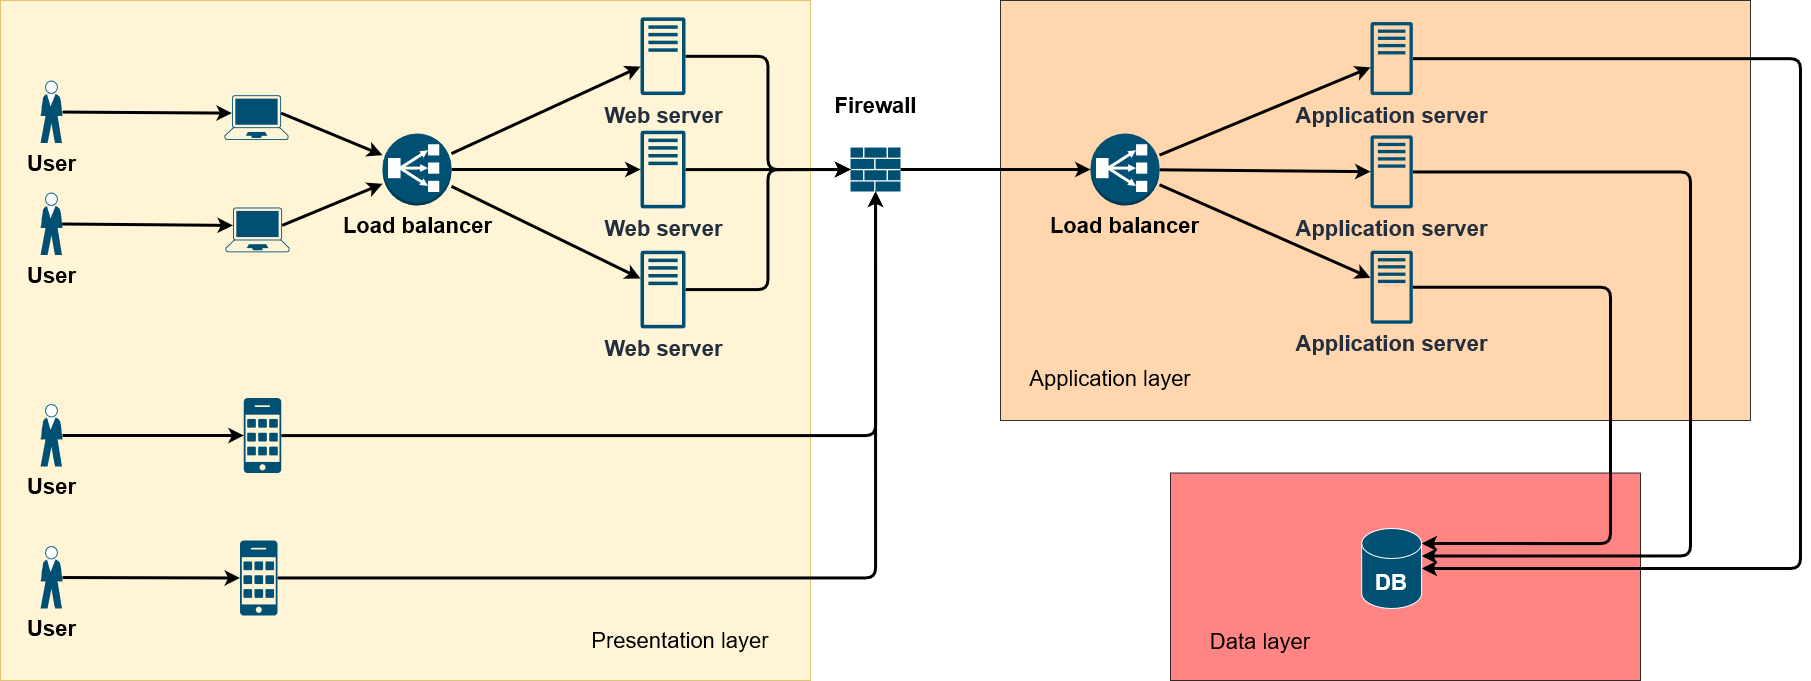
\includegraphics[width=\textwidth,height=\textheight,keepaspectratio]{Images/architectureDesignDiagram.png}
    \caption{Architecture of the application}
    \label{fig:architectue_diagram}
\end{figure}

As shown in figure \ref{fig:architectue_diagram} the application is divided into 3 layers and 4 tiers. Users can access the service
both from a mobile app or web interface. The figure shows the division of the different layers. Since the application follows the 
REST standard the servers are stateless. There will be a more precise description of the components in the following sections.

\subsection{Component View}
\begin{figure}[H]
    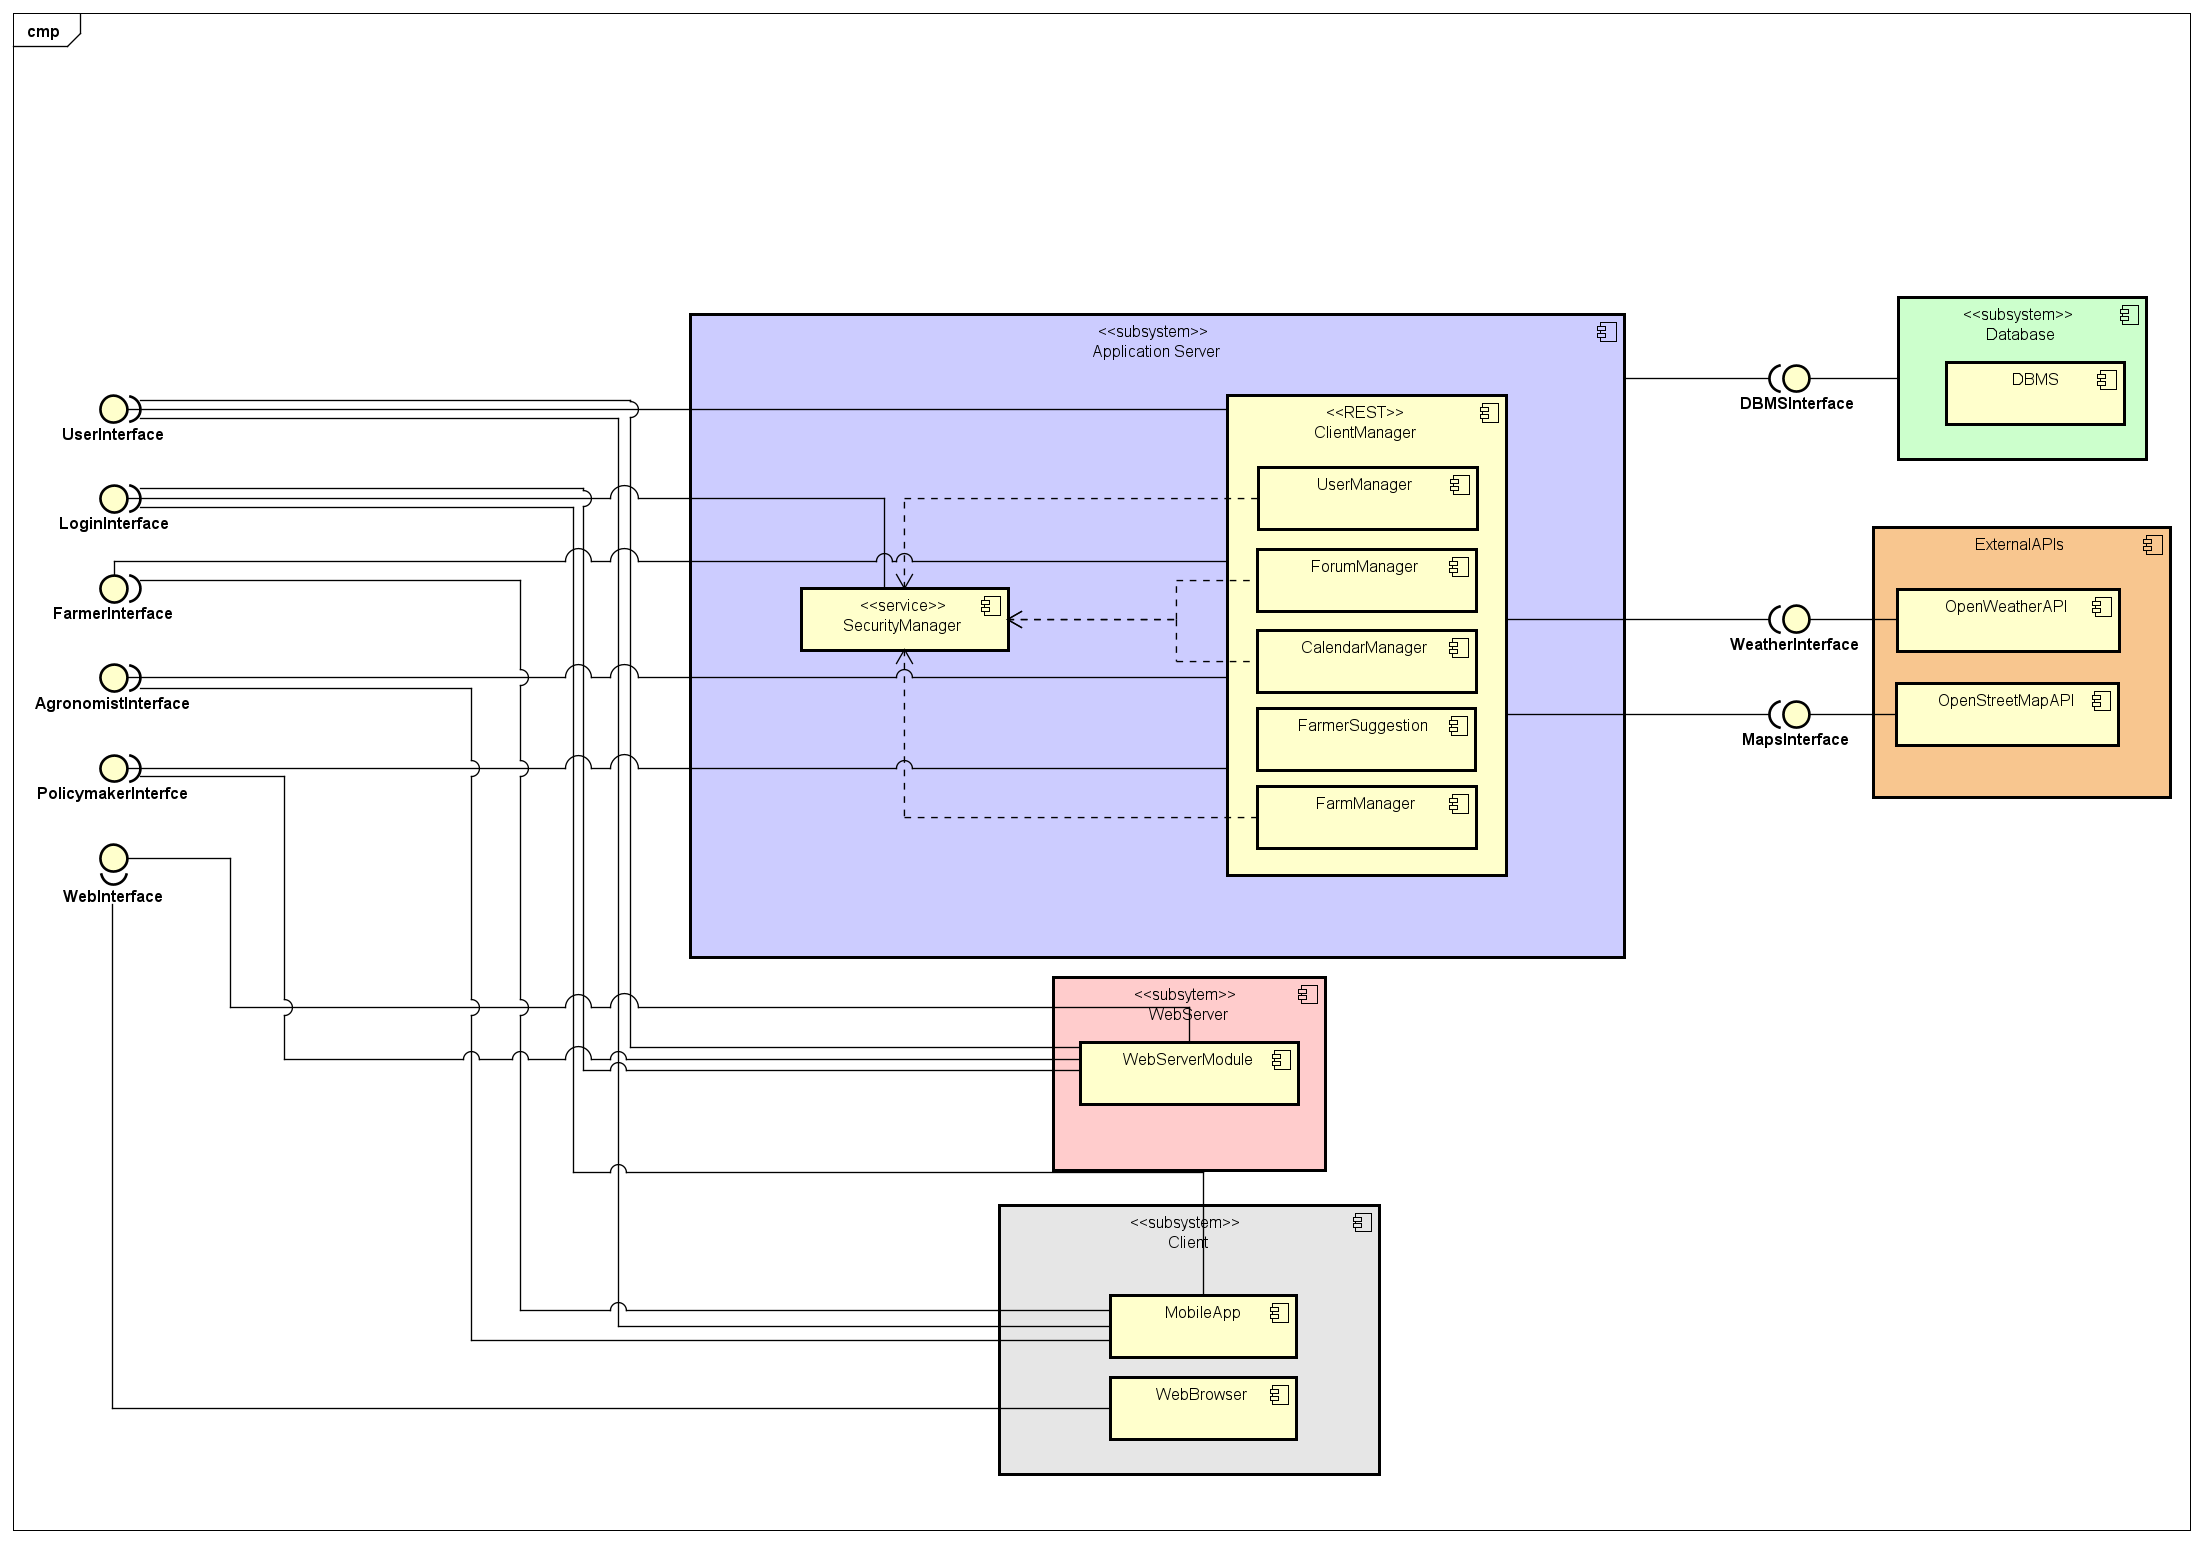
\includegraphics[width=\textwidth,height=\textheight,keepaspectratio]{Images/ComponentDiagram.png}
    \caption{Component Diagram}
    \label{fig:component_diagram}
\end{figure}

Figure \ref{fig:component_diagram}  represents in detail the layers described before. The web server has the function to
route the browser requests to the application server and send back its responses.

\begin{itemize}
    \item \textbf{Client Manager}\\
        This module handles all the requests made by the client. In the beginning,
        when the client is not logged in, the module offers (through
        the user manager) a loginInterface that allows the client to register and log in. After the login the module
        provide an interface based on the role of the user: FarmInterface for the farmer, AgronomistInterface for the agronomist,
        PolicymakerInterface for the policymaker.

    \item \textbf{User Manager}\\
        This module provides all the functionalities needed to manage the user. It includes signup and login as well as role checking 
        operation and information retrieving.
           
    \item \textbf{Forum Manager}\\
        This module provides all the functionalities through the ForumInterface for managing and using the forum. 
        It includes operations for creating and replying to a discussion on the forum.

    \item \textbf{Calendar Manager}\\
        This Module provides all the functionalities needed for the Agronomist to manage his calendar. In particular, it provides
        through, the AgronomistInterface, the possibility to add or remove an appointment, to confirm the daily plan and to check
        that each farm has at least two visits per year.

    \item \textbf{Farmer Suggestion}\\
        This module handles the creation and delivery of personalized suggestions to the Farmer. 

    \item \textbf{Farm Manager}\\
        This module provides to the Farmer all the functionalities for giving information about their farm. 
        It provides the possibility to add information about the harvest and to request help from the Agronomist.

    \item \textbf{Security Manager}\\
        This module handles all the security issues.
\end{itemize}

\newpage
\subsection{Deployment diagram}
\begin{figure}[H]
    \begin{center}
        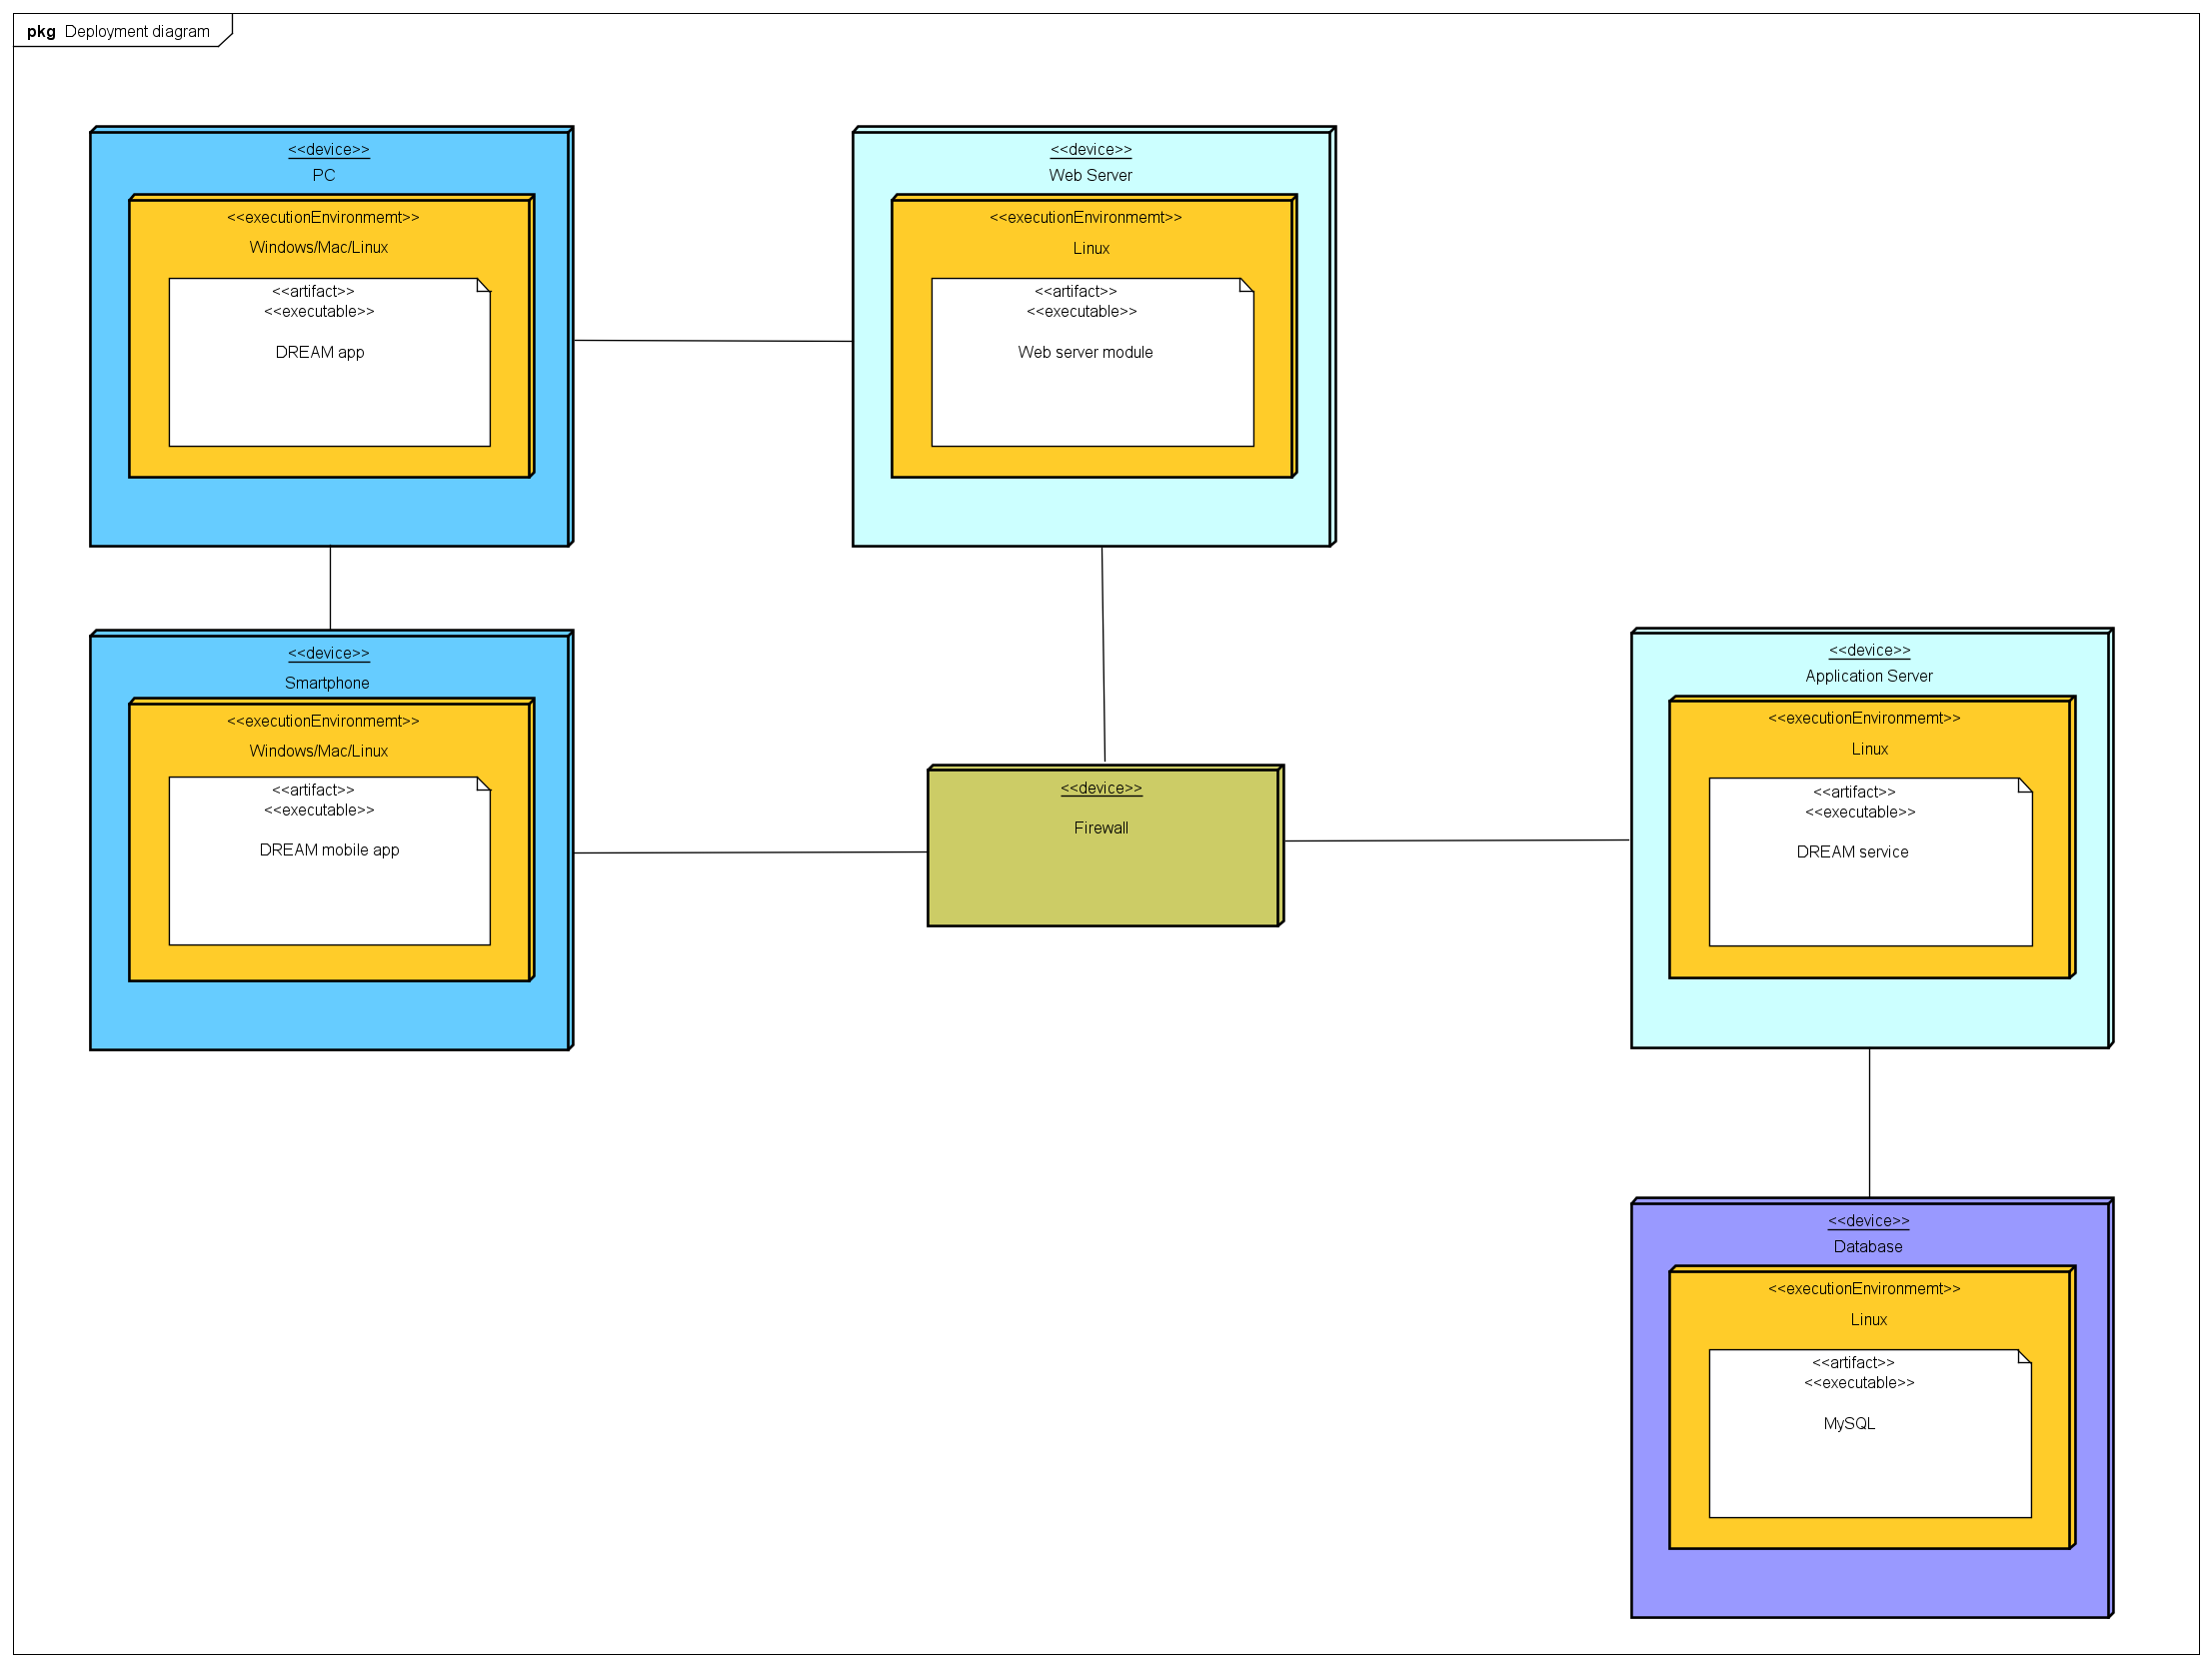
\includegraphics[width=\textwidth]{Images/DeploymentDiagram.png}
        \caption{Deployment Diagram}
    \end{center}
\end{figure}

The deployment diagram in figure shows the needed components for correct system behavior.
Each device owns its Operating System where the software runs. Firewall ensures application security.
\newline The tiers in the image are the following:
\begin{itemize}
    \item \textbf{Tier 1:} it is the client machine, which can be a computer with a web browser or the mobile
    application.
    \item \textbf{Tier 2:} includes the replicated web servers, which do not execute any business logic, but simply receive
    requests from the client, route them to the application servers and serve an HTML back to the client.
    \item \textbf{Tier 3:} it includes the application servers that contain the whole application layer and communicate to the data tier.
    \item \textbf{Tier 4:} it contains the DBMS servers that store and manage data, according to the instructions given by the application servers.
\end{itemize}

\newpage

\subsection{Component Interfaces}
\begin{figure}[H]
    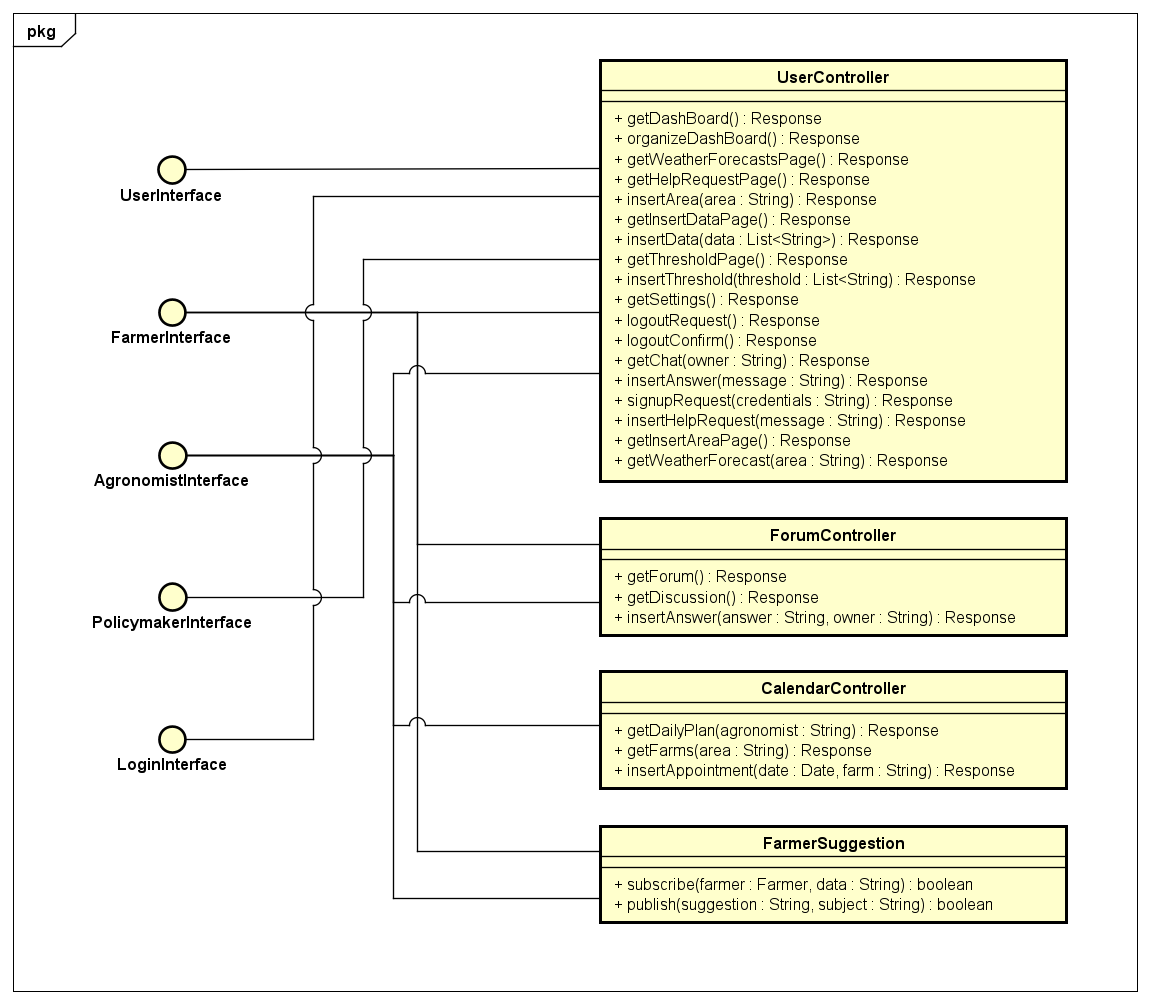
\includegraphics[width=\textwidth,height=\textheight,keepaspectratio]{Images/InterfaceDiagram.png}
    \caption{Interface Diagram}
    \label{fig:interface_diagram}
\end{figure}
Figure \ref{fig:interface_diagram} shows the main interfaces of the system.\newline
The \textbf{UserInterface} provides the functionalities common to all users, it is realized through just one controller the \textbf{UserController}. \newline
The \textbf{FarmerInterface} provides all the specific functionalities of the farmer and it is realized through three controllers: \textbf{UserController}, \textbf{ForumController}, \textbf{FarmerSuggestion}.\newline
The \textbf{AgronomistInterface} provides all the specific functionalities of the agronomist and it is realized through four controllers     :
\textbf{UserController}, \textbf{ForumController}, \textbf{FarmerSuggestion},\textbf{CalendarController}.\newline
The \textbf{PolicymakerInterface} provides all the specific functionalities of the policymaker and it is realized through one controller:
\textbf{UserController}.\newline
The \textbf{LoginInterface} provides all the functionalities for login and signup and it is realized through \textbf{UserController}.


\subsection{Logical Description of Data}
\begin{figure}[H]
    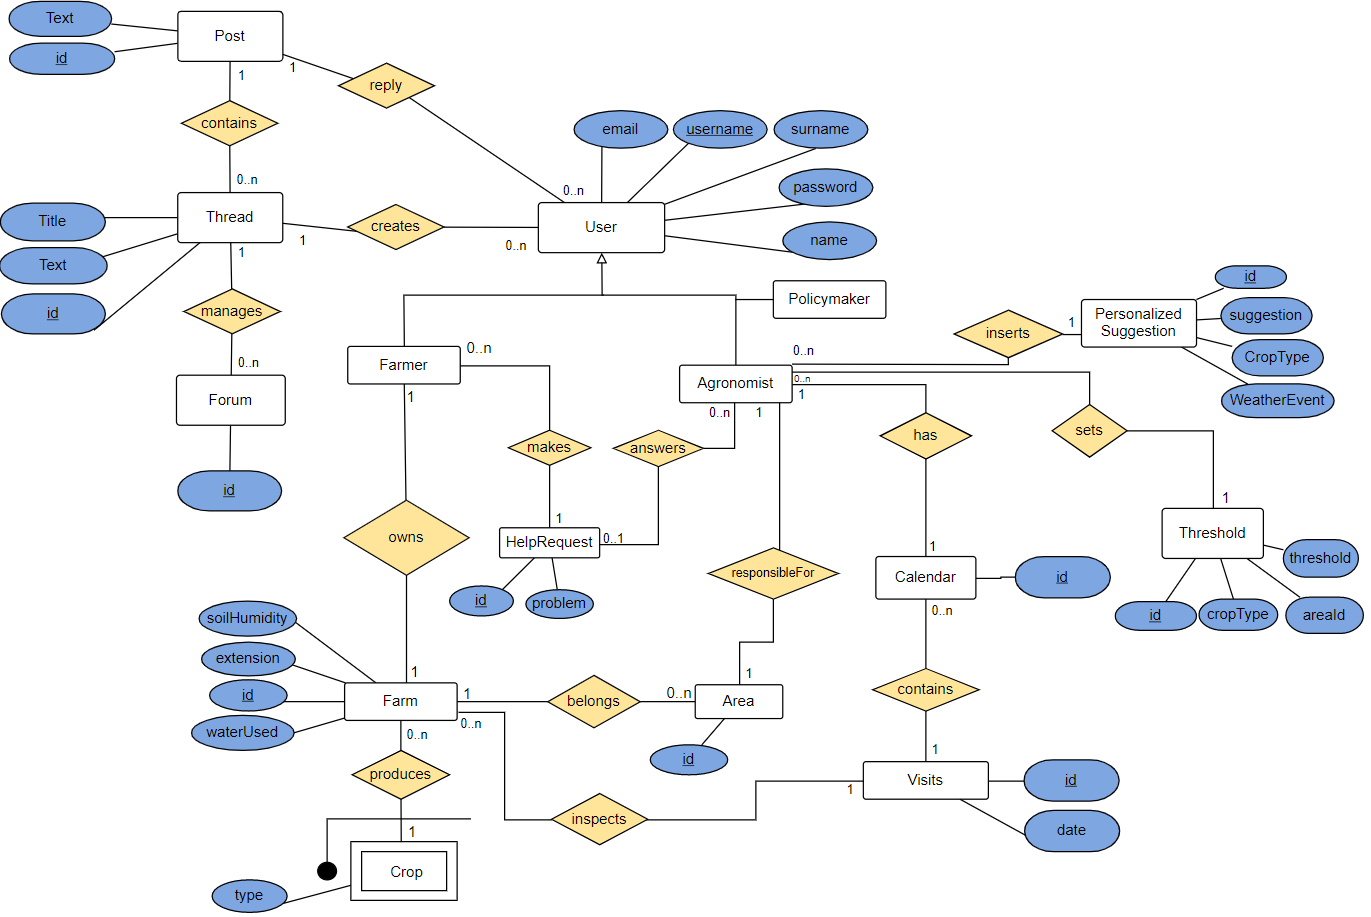
\includegraphics[width=\textwidth,height=\textheight,keepaspectratio]{Images/erDiagram.png}
    \caption{ER Diagram}
    \label{fig:er_diagram}
\end{figure}
Figure \ref{fig:er_diagram} shows a logical representation of the data that will be stored in the database of the system.


%------------------------------------------------------------------------------------------------------------------------------------------------
\clearpage
{\color{Blue}{\section{User Interface Design}}}
\label{sect:interface}
This section aims to describe the flow of the main functionalities of the application.\\
We used some mockups already presented in the RASD, but more have been created and added to
this part to cover all the main functionalities of the application. In addition, we chose
to show only the mobile application because, in our opinion, Users would interact mostly with it.
We want to remember that the application will work also on web browsers for all types of users,
but the design and the interfaces of the web app will derive from these.
\\
\bigskip
\subsection{User Mobile Interface}
The following images represent the flow of the functionalities common to all the users of the application.\\
\begin{center}
    \begin{figure}[H]
        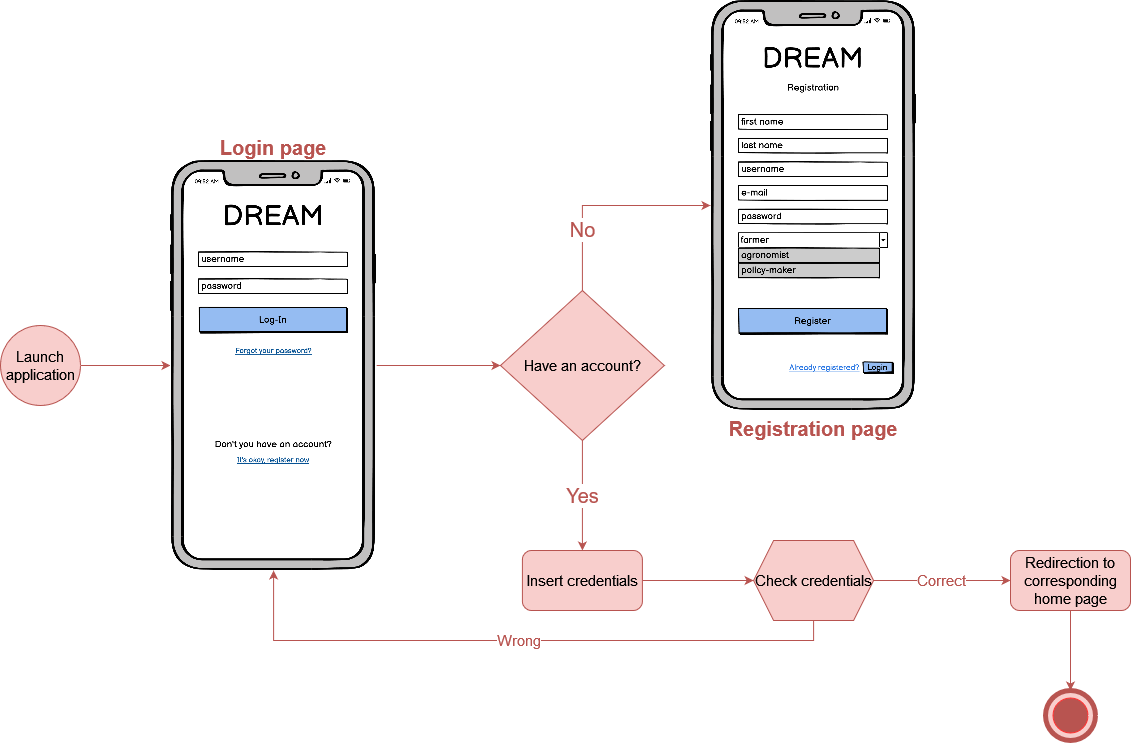
\includegraphics[width=\textwidth]{Images/UserInterface/Diagram/login.drawio.png}
        \caption{Sign Up \& Sign In}
    \end{figure}
\end{center}
\newpage

\begin{center}
    \begin{figure}[H]
        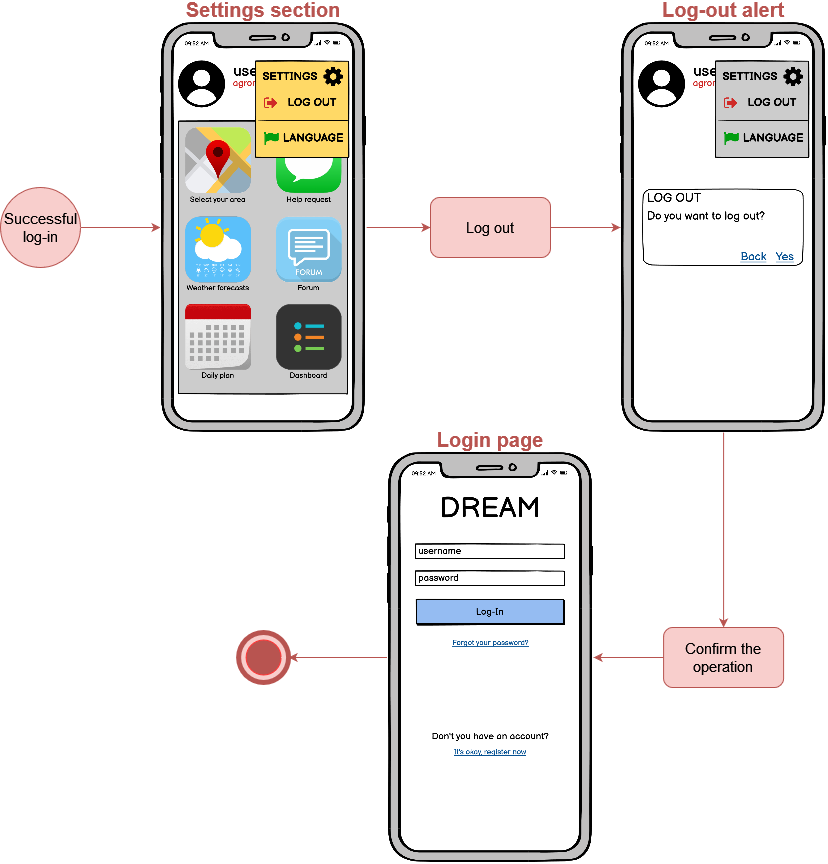
\includegraphics[width=\textwidth]{Images/UserInterface/Diagram/logout.drawio.png}
        \caption{Logout}
    \end{figure}
\end{center}
\newpage

\subsection{Farmer Mobile Interface}
\begin{center}
    \begin{figure}[H]
        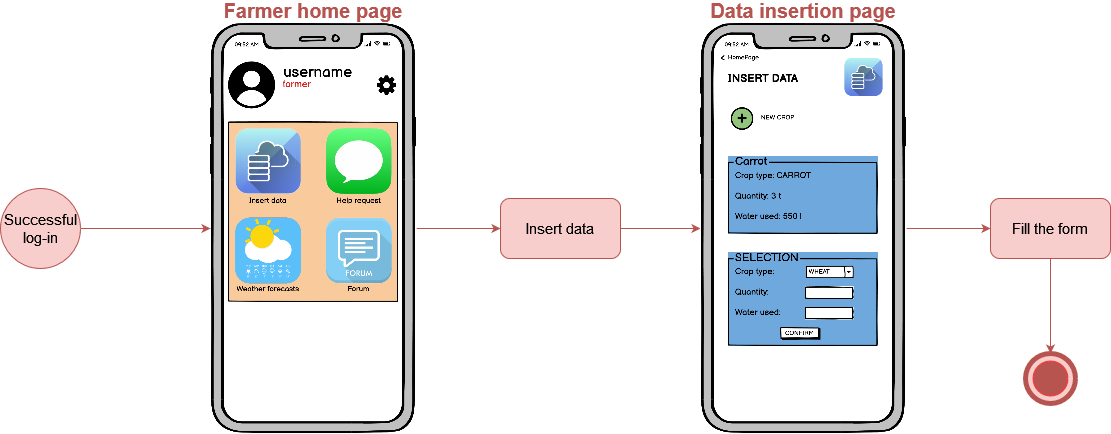
\includegraphics[width=\textwidth]{Images/UserInterface/Diagram/farmerData.drawio.png}
        \caption{Data insertion}
    \end{figure}
\end{center}

\begin{center}
    \begin{figure}[H]
        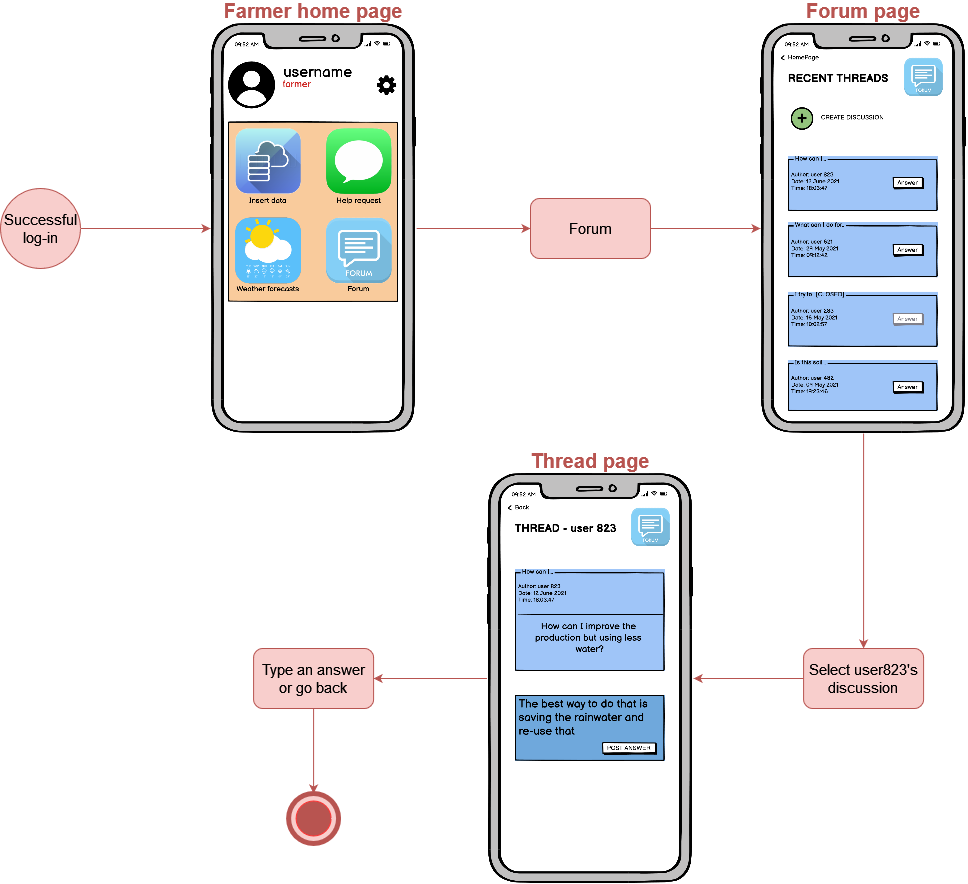
\includegraphics[scale=0.42]{Images/UserInterface/Diagram/farmerForum.drawio.png}
        \caption{Forum functionalities}
    \end{figure}
\end{center}

\begin{center}
    \begin{figure}[H]
        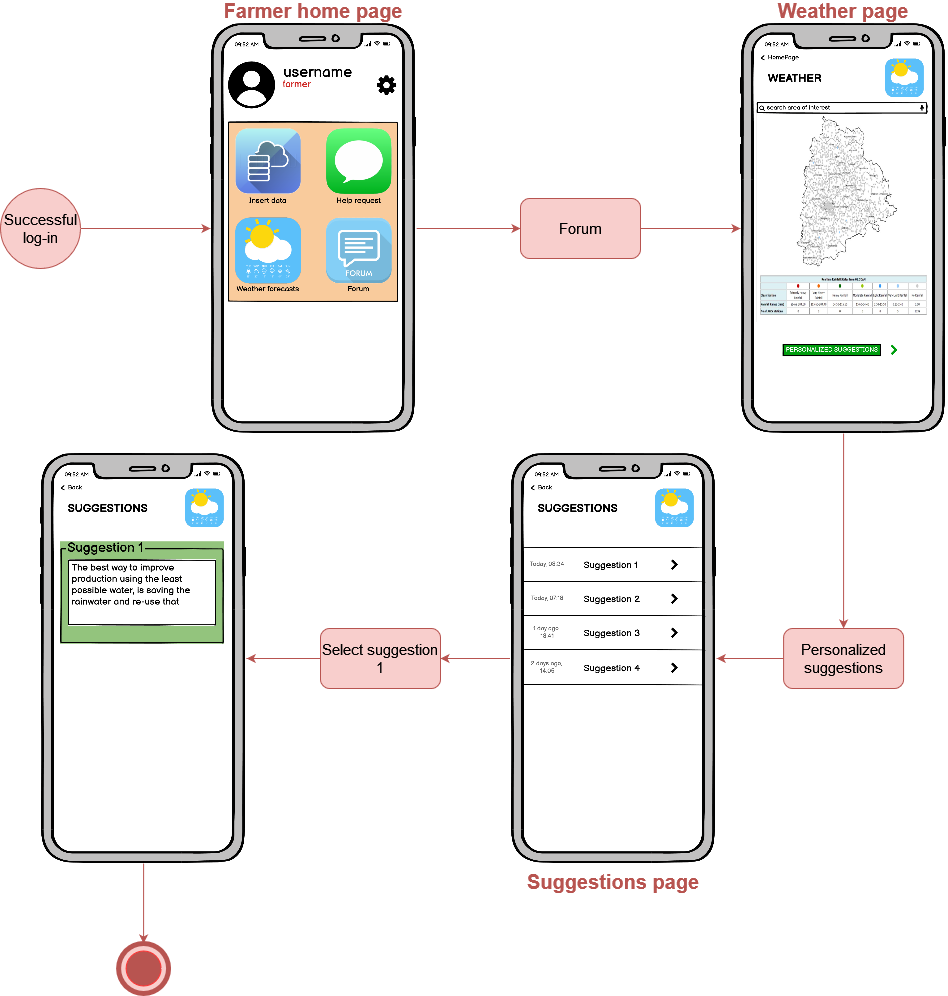
\includegraphics[width=\textwidth]{Images/UserInterface/Diagram/farmerWeather.drawio.png}
        \caption{Weather forecasts and personalized suggestions}
    \end{figure}
\end{center}
\newpage

\begin{center}
    \begin{figure}[H]
        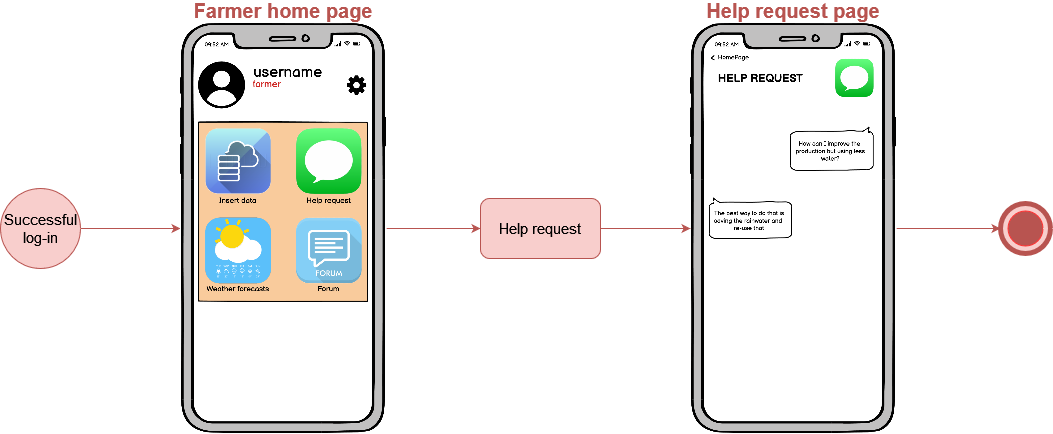
\includegraphics[width=\textwidth]{Images/UserInterface/Diagram/HelpRequestFarmerSide.drawio.png}
        \caption{Help request}
    \end{figure}
\end{center}
\bigskip
\bigskip

\subsection{Agronomist Mobile Interface}
\begin{center}
    \begin{figure}[H]
        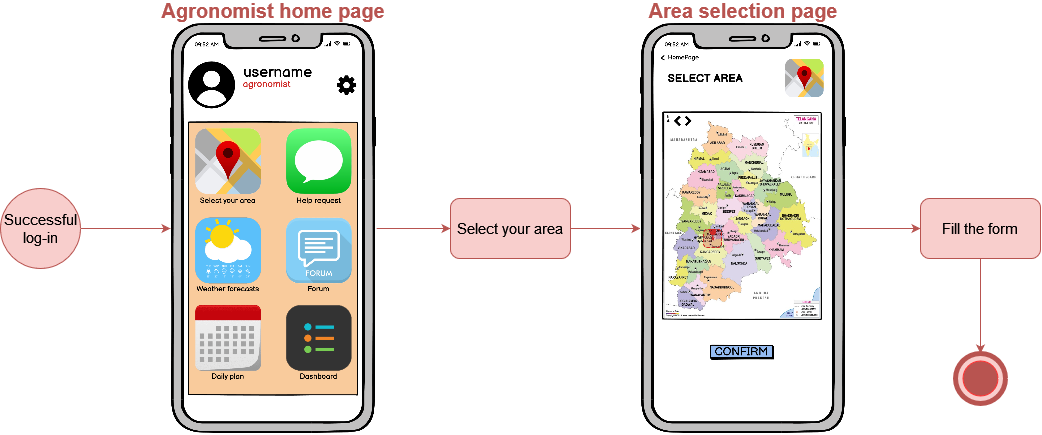
\includegraphics[width=\textwidth]{Images/UserInterface/Diagram/selectArea.drawio.png}
        \caption{Area of responsibility selection page}
    \end{figure}
\end{center}
\newpage

\begin{center}
    \begin{figure}[H]
        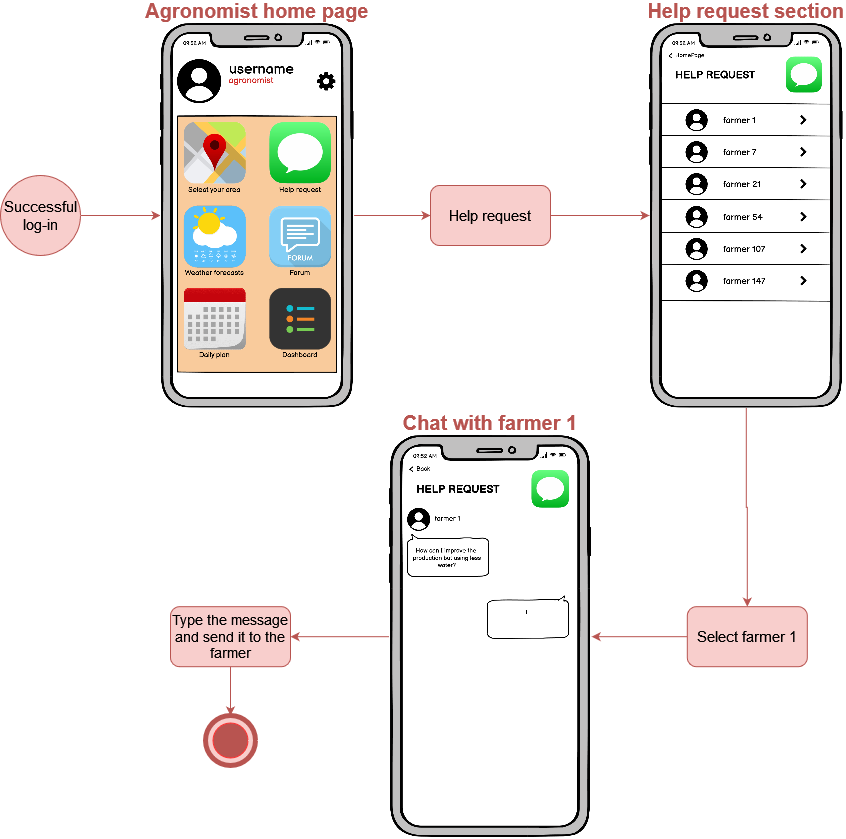
\includegraphics[width=\textwidth]{Images/UserInterface/Diagram/appChart.drawio.png}
        \caption{Help request}
    \end{figure}
\end{center}
\newpage

\begin{center}
    \begin{figure}[H]
        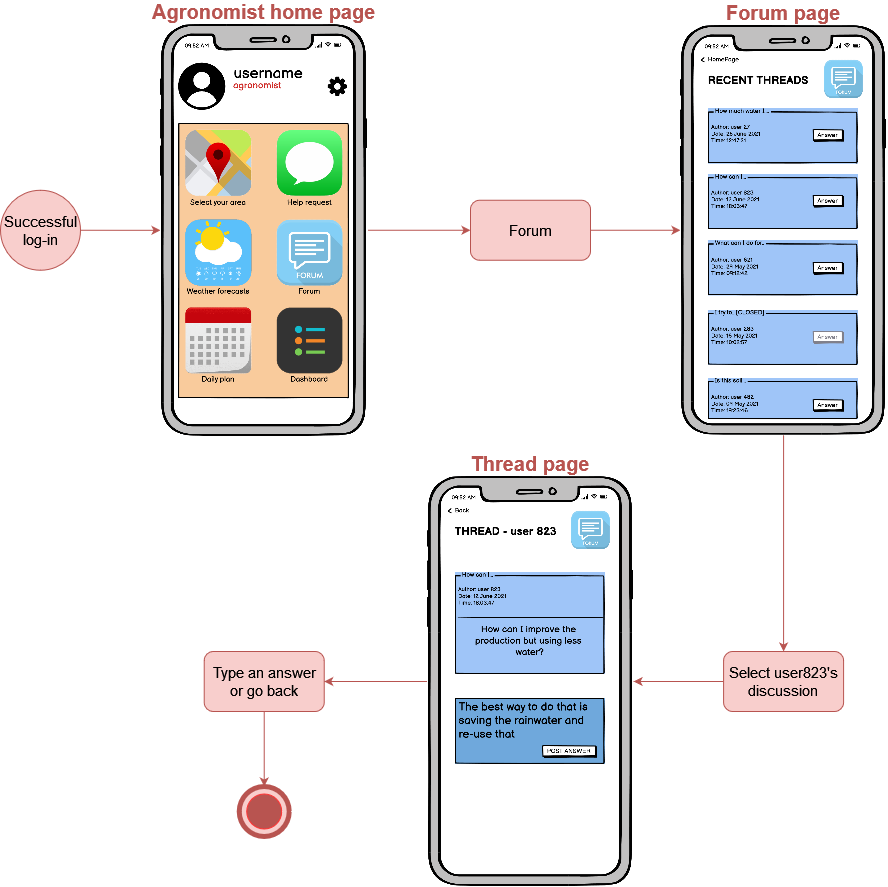
\includegraphics[width=\textwidth]{Images/UserInterface/Diagram/agronomistForum.drawio.png}
        \caption{Forum functionalities}
    \end{figure}
\end{center}
\newpage

\begin{center}
    \begin{figure}[H]
        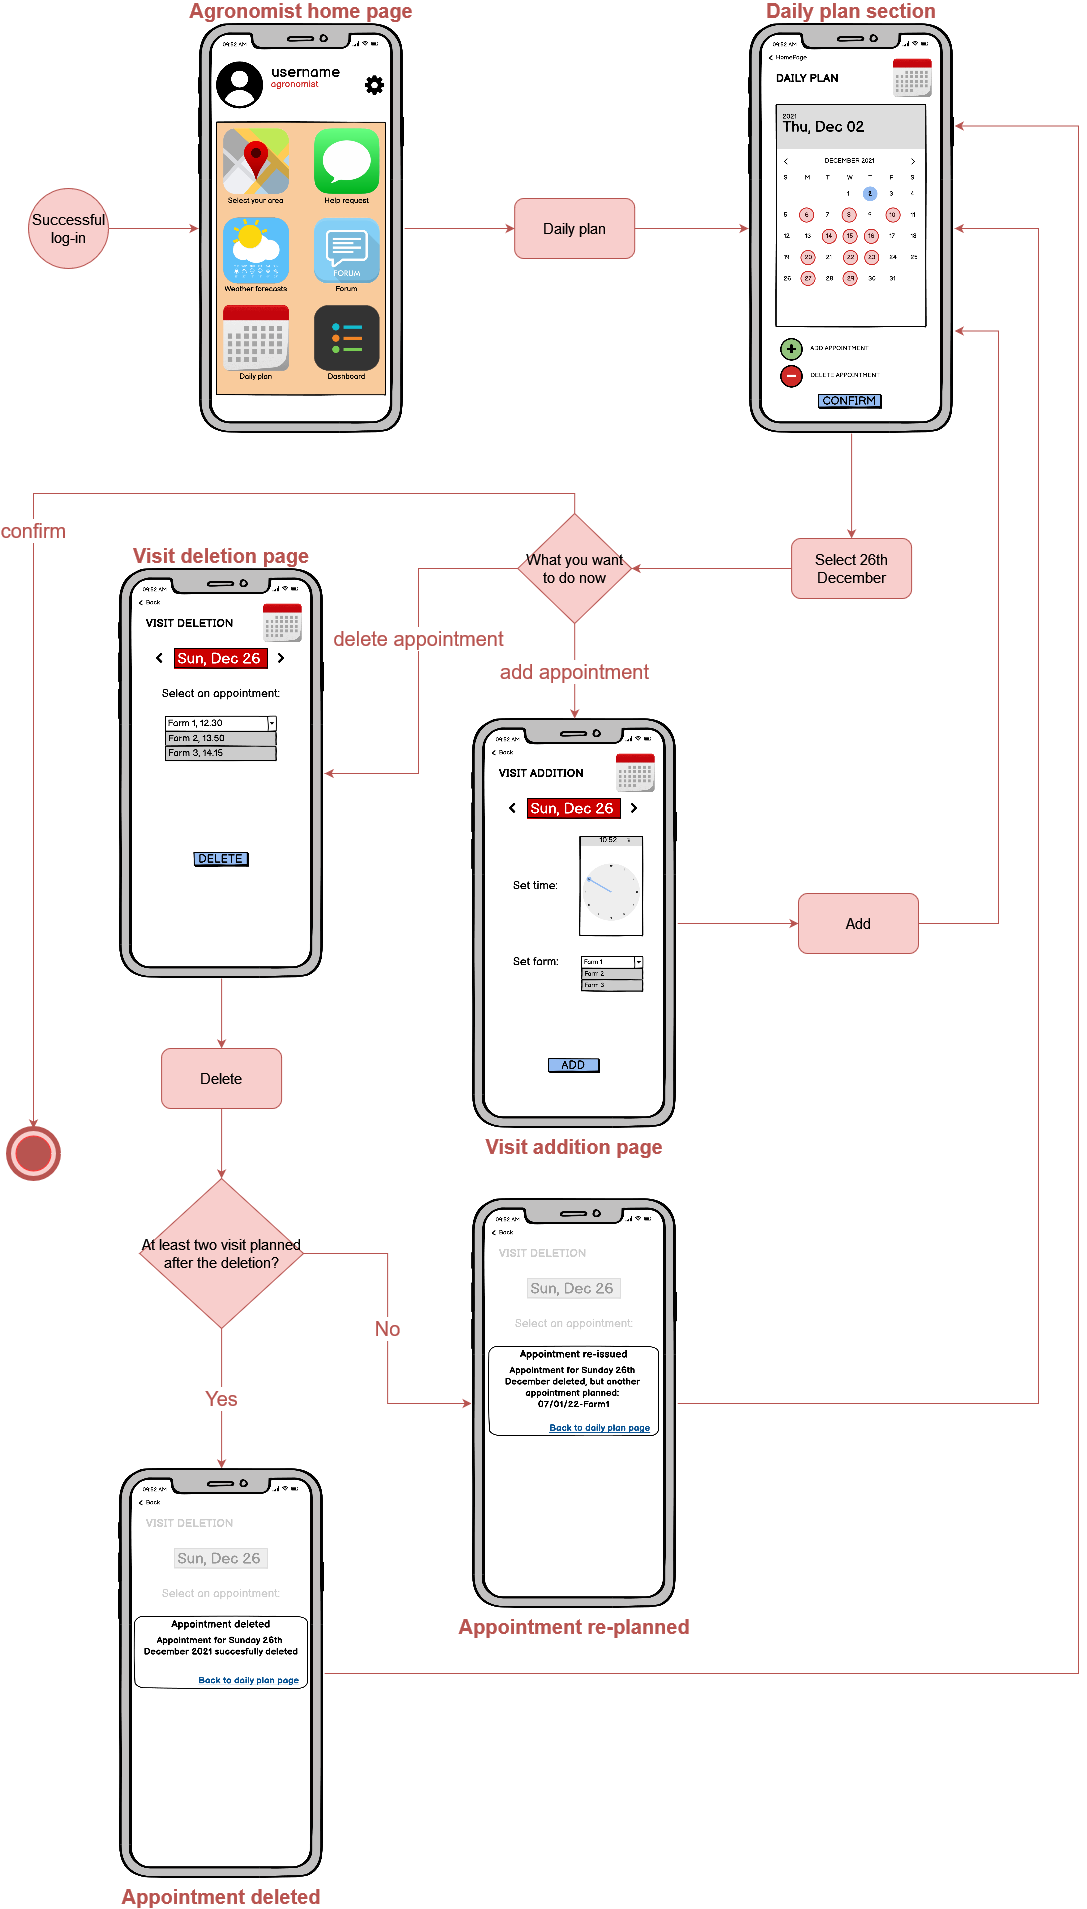
\includegraphics[scale=0.34]{Images/UserInterface/Diagram/DailyPlan.drawio.png}
        \caption{Daily plan functionalities}
    \end{figure}
\end{center}

\begin{center}
    \begin{figure}[H]
        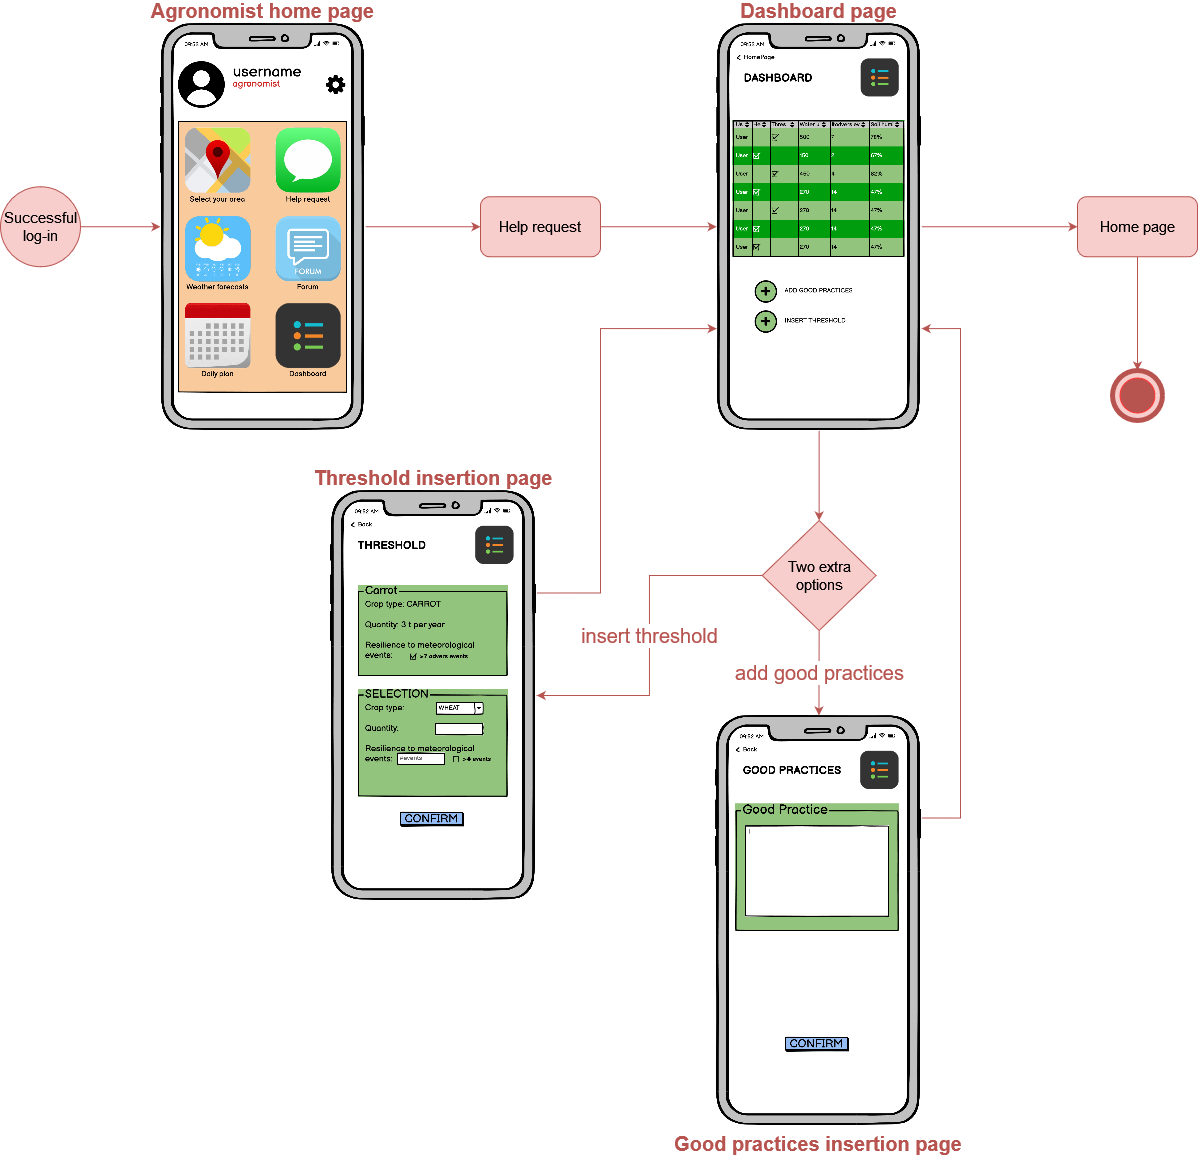
\includegraphics[width=\textwidth]{Images/UserInterface/Diagram/dashboard.drawio.png}
        \caption{Dashboard}
    \end{figure}
\end{center}
\newpage







%------------------------------------------------------------------------------------------------------------------------------------------------
\clearpage
{\color{Blue}{\section{Requirements Traceability}}}
\label{sect:requirementsTraceability}
This section will show the traceability between requirements and modules described in component diagram.
In the table some abbreviation have been used:\newline
\begin{itemize}
    \item UM: UserManager
    \item FM: ForumManager
    \item CM: CalendarManager
    \item FS: FarmerSuggestion
    \item FAM: FarmManager
    \item MS: MeteoService
\end{itemize}

\begin{table}[]
    \begin{tabular}{|l|l|l|l|l|l|l|l|}
    \hline
        & UM & FM & CM & FS & FAM & MS & DBMS \\ \hline
    R1  & X  &    &    & X  &     &    & X    \\ \hline
    R2  &    &    &    &    & X   & X  & X    \\ \hline
    R3  &    &    &    &    &     & X  & X    \\ \hline
    R4  & X  &    &    &    &     &    & X    \\ \hline
    R5  & X  &    &    &    & X   &    & X    \\ \hline
    R6  & X  &    &    & X  &     &    & X    \\ \hline
    R7  & X  & X  &    &    &     &    & X    \\ \hline
    R8  & X  & X  &    &    &     &    & X    \\ \hline
    R9  & X  &    &    &    &     &    & X    \\ \hline
    R10 & X  &    &    & X  &     &    & X    \\ \hline
    R11 &    &    &    &    &     & X  & X    \\ \hline
    R12 & X  &    &    &    &     & X  & X    \\ \hline
    R13 &    & X  &    &    &     &    & X    \\ \hline
    R14 & X  &    & X  &    & X   &    & X    \\ \hline
    R15 & X  &    & X  &    &     &    & X    \\ \hline
    R16 &    &    & X  &    &     &    &      \\ \hline
    R17 & X  &    &    &    &     &    & X    \\ \hline
    R18 & X  &    &    &    &     &    & X    \\ \hline
    R19 & X  &    &    & X  &     &    & X    \\ \hline
    R20 & X  & X  &    &    &     &    & X    \\ \hline
    R21 & X  &    &    &    &     & X  & X    \\ \hline
    R22 & X  &    & X  &    &     &    & X    \\ \hline
    R23 & X  &    & X  &    &     &    &      \\ \hline
    R24 & X  &    &    &    &     &    & X    \\ \hline
    R25 & X  &    &    &    &     &    & X    \\ \hline
    R26 & X  &    &    &    &     &    & X    \\ \hline
    R27 & X  &    &    & X  &     &    & X    \\ \hline
    R28 & X  & X  &    &    &     &    & X    \\ \hline
    R29 &    &    &    &    & X   &    & X    \\ \hline
    R30 &    &    &    &    & X   &    & X    \\ \hline
    R31 &    &    &    &    & X   &    & X    \\ \hline
    R32 & X  &    &    &    &     &    & X    \\ \hline
    R33 & X  &    &    &    &     &    & X    \\ \hline
    R34 & X  &    &    &    &     &    & X    \\ \hline
    R35 & X  &    &    &    &     &    & X    \\ \hline
    R36 & X  &    &    &    &     &    & X    \\ \hline
    R37 & X  &    &    &    &     &    & X    \\ \hline
    \end{tabular}
    \end{table}

%------------------------------------------------------------------------------------------------------------------------------------------------
\clearpage
{\color{Blue}{\section{Implementation, Integration and Test Plan}}}
\label{sect:implementation}
\subsection{Recommended Implementation}
The system will be composed by:
\begin{itemize}
    \item Client : it can be a mobile or a web application
    \item Web Server
    \item Application Server
    \item Database
    \item External APIs (such as OpenWeather and OpenStreetMap)
\end{itemize}

\subsection{Implementation Plan}
The above components should be developed following a bottom-up logic, therefore, avoiding difficulties in integration and testing.\bigskip

Firstly some basic functionalities should be completely developed so that the other related functionalities can then be added and tested.\newline
The first module that should be written is the one that provides authentication and account creation interfacing with the DBMS. 
Because of that, the system can soon reach partial functionality.\newline 
Then can be developed the web application using the REST API which includes all the main functionalities of the users.
The next steps to complete the system should be:
\begin{itemize}
    \item The client interfaces
    \item The coupling with external APIs
\end{itemize}

\subsection{Testing Plan}
Testing should be done throughout all stages of development, following a bottom up approach.\bigskip

Unit tests should be written starting from the basic component so that tests for other components that
use them can be written relying on the fact that the subcomponents are already tested. This speeds up
debugging since it’s easy to locate at which level of the component hierarchy there is a problem.

\subsection{Integration Plan}
In this section there is be a description about how the components are integrated and communicate.
The first component to build is the DBMS, followed by the main application components that exploit it.
After this, we have to integrate the API communication between the System and the external services that will be used.
t this point it is possible to integrate the User Manager, which permits to Users to exploit all the functionalities.
Finally, it is possible to integrate the web server module with the mobile application module and the browser with the web server module.


%------------------------------------------------------------------------------------------------------------------------------------------------
\clearpage
{\color{Blue}{\section{Effort Spent}}}
\label{sect:effort}
\begin{table}[H]
    \centering
    \begin{tabular}{|l|l|l|}
        \multicolumn{3}{c}{\textbf{Lorenzo Iovine}}                   \\
        \hline
        \textbf{Date} & \textbf{Hours} & \textbf{Description}          \\\hline
        2021-11-29    & 7h             & Introduction, Purpose, Scope \& Goals                  \\\hline
        2021-11-30    & 5h             & UML diagram, statecharts \& World and the Machine      \\\hline
        2021-12-01    & 7h             & Product functions                                      \\\hline
        2021-12-02    & 3h             & Product functions, User characteristics \& Assumptions \\\hline
        2021-12-02    & 4h             & Mockups                                                \\\hline
        2021-12-03    & 4h             & Use cases                                              \\\hline
        2021-12-04    & 2h             & Use cases                                              \\\hline
        2021-12-04    & 4h             & Sequence diagram                                       \\\hline
        2021-12-05    & 3h             & Review                                                 \\\hline
        2021-12-06    & 5h             & Review \& Alloy                                        \\\hline
        2021-12-07    & 3h             & Alloy                                                  \\\hline\hline
                      & 47h            &                                                        \\\hline
    \end{tabular}
\end{table}
\begin{table}[H]
    \centering
    \begin{tabular}{|l|l|l|}
        \multicolumn{3}{c}{\textbf{Nicola Landini}}                      \\
        \hline
        \textbf{Date} & \textbf{Hours} & \textbf{Description}                                   \\\hline
        2021-11-29    & 7h             & Introduction, Purpose, Scope \& Goals                  \\\hline
        2021-11-30    & 5h             & UML diagram, statecharts \& World and the Machine      \\\hline
        2021-12-01    & 7h             & Product functions                                      \\\hline
        2021-12-02    & 3h             & Product functions, User characteristics \& Assumptions \\\hline
        2021-12-02    & 4h             & Mockups                                                \\\hline
        2021-12-03    & 4h             & Customer Interfaces                                    \\\hline
        2021-12-04    & 2h             & Customer Interfaces                                    \\\hline
        2021-12-04    & 4h             & Sequence diagram                                       \\\hline
        2021-12-05    & 3h             & Review                                                 \\\hline
        2021-12-06    & 5h             & Review \& Alloy                                        \\\hline
        2021-12-07    & 3h             & Alloy                                                  \\\hline\hline
                      & 47h            &                                                        \\\hline
    \end{tabular}
\end{table}
\begin{table}[H]
    \centering
    \begin{tabular}{|l|l|l|}
        \multicolumn{3}{c}{\textbf{Francesco Leone}}                      \\
        \hline
        \textbf{Date} & \textbf{Hours} & \textbf{Description}              \\\hline
        2021-11-29    & 7h             & Introduction, Purpose, Scope \& Goals                  \\\hline
        2021-11-30    & 5h             & UML diagram, statecharts \& World and the Machine      \\\hline
        2021-12-01    & 7h             & Product functions                                      \\\hline
        2021-12-02    & 3h             & Product functions, User characteristics \& Assumptions \\\hline
        2021-12-02    & 4h             & Requirements                                           \\\hline
        2021-12-03    & 4h             & Use cases                                              \\\hline
        2021-12-04    & 2h             & Use cases                                              \\\hline
        2021-12-04    & 4h             & Sequence diagram                                       \\\hline
        2021-12-05    & 3h             & Review                                                 \\\hline
        2021-12-06    & 5h             & Review \& Alloy                                        \\\hline
        2021-12-07    & 3h             & Alloy                                                  \\\hline\hline
                      & 47h            &                                                        \\\hline
    \end{tabular}
\end{table}

%------------------------------------------------------------------------------------------------------------------------------------------------




\end{document}
